\documentclass{birkjour}

\usepackage{amsmath}
\usepackage{amssymb}
\usepackage{amsthm}
\usepackage{graphicx}
\usepackage{float}

\newtheorem{thm}{Theorem}[section]
 \newtheorem{cor}[thm]{Corollary}
 \newtheorem{lem}[thm]{Lemma}
 \newtheorem{prop}[thm]{Proposition}
 \theoremstyle{definition}
 \newtheorem{defn}[thm]{Definition}
 \theoremstyle{remark}
 \newtheorem{rem}[thm]{Remark}
 \newtheorem*{ex}{Example}
 \numberwithin{equation}{section}

\newcommand{\G}{\mathbb{G}}
\newcommand{\V}{\mathbb{V}}
\newcommand{\Vb}{\mathbb{\overline{V}}}
\newcommand{\W}{\mathbb{W}}
\newcommand{\R}{\mathbb{R}}

\newcommand{\Alpha}{A}
%\Omega is already defined

\newcommand{\nvao}{o}
\newcommand{\nvai}{\infty}
\newcommand{\nvaob}{\overline{o}}
\newcommand{\nvaib}{\overline{\infty}}

\newcommand{\eminus}{e_{-}}
\newcommand{\eplus}{e_{+}}
\newcommand{\eminusb}{\overline{e}_{-}}
\newcommand{\eplusb}{\overline{e}_{+}}

\begin{document}

\title{An Extension Of The Quadric Model}

\author{Spencer T. Parkin}
\address{%
2113 S. Claremont Dr.\\
Bountiful, Utah  84010\\
USA}
\email{spencer.parkin@gmail.com}

\numberwithin{equation}{section}

\subjclass{Primary 14J70; Secondary 14J29}

\keywords{Quadric Surface, Quartic Surface, Geometric Algebra, Quadric Model, Conformal Model}

%\dedicatory{To Melinda and Naomi}

\begin{abstract}
An extension of the quadric model set forth in \cite{Parkin12} is
found in which the rigid body motions are represented by
versors applicable to any quadric surface.
Extending the model yet further to include
a specific form of quartic surface, we find that the versors of
the conformal model may be used to transform any such surface.
Results of a computer program implementing this model are presented.
\end{abstract}

\maketitle

\section{Introduction}

In the original paper \cite{Parkin12}, a model for quadric surfaces was
presented based upon the ideas of projective geometry.  What was unfortunate
about this model, however, was its lack of support for the rigid body transformations.  It was
predicted in the conclusion of that paper that a better model for quadric
surfaces may exist that is more like the conformal model of geometric algebra.
The present paper details what may be such a model.  We'll find that the rigid
body transformations can be incorporated into the model by using an alternative
method of encoding the quadric form.  An extension to the quadric form
will then allow us to support the conformal transformations at the expense of
expanding our model to necessarily include a specific form of quartic surfaces.  Both extensions
of the original quadric model will use the same geometric algebra.

\section{The Geometric Algebra}

We begin here with a description of the structure of the geometric algebra upon
which our model will be imposed.  This
geometric algebra will contain the following vector spaces.
\begin{equation}\label{equ_vector_spaces}
\begin{array}{ll}
\mbox{Notation} & \mbox{Basis} \\
\hline
\V^e & \{e_i\}_{i=1}^n \\
\V^{\nvao} & \{\nvao\}\cup\{e_i\}_{i=1}^n \\
\V^{\nvai} & \{e_i\}_{i=1}^n\cup\{\nvai\} \\
\V & \{\nvao\}\cup\{e_i\}_{i=1}^n\cup\{\nvai\}
\end{array}
\end{equation}
The set of vectors $\{e_i\}_{i=1}^n$ forms an orthonormal set of basis
vectors for the $n$-dimensional Euclidean vector space $\V^e$, which we'll
use to represent $n$-dimensional Euclidean space.
The vectors $\nvao$ and $\nvai$ are the familiar null-vectors representing the
points at origin and infinity taken from the conformal model of geometric algebra.
An inner-product table for these basis vectors is given as follows, where
$1\leq i<j\leq n$.
\begin{equation}
\begin{array}{c|cccc}
\cdot & \nvao & e_i & e_j & \nvai \\
\hline
\nvao & 0 & 0 & 0 & -1 \\
e_i & 0 & 1 & 0 & 0 \\
e_j & 0 & 0 & 1 & 0 \\
\nvai & -1 & 0 & 0 & 0
\end{array}
\end{equation}
We will now let $\G(\V)$ denote the Minkowski geometric algebra generated by $\V$.
For each vector space in table \eqref{equ_vector_spaces}, we will let an over-bar
above this vector space denote an identical copy of that vector space.  The vector
space $\W$ will denote the smallest vector space containing each of $\V$ and $\Vb$
as vector subspaces.  In symbols, one may write
\begin{equation}
\G(\W) = \G(\V)\oplus\G(\Vb)
\end{equation}
to illustrate the structure of $\G(\W)$ in terms of its two isomorphic Minkowski
geometric sub-algebras $\G(\V)$ and $\G(\Vb)$.

We will use over-bar notation to distinguish between vectors taken from $\V$
with vectors taken from $\Vb$.  Though not necessary, we can work exclusively
in $\G(\V)$ by defining the over-bar notation as an outermorphic ismorphism between
$\G(\V)$ and $\G(\Vb)$.  Doing so, we see that for any element $E\in\G(\V)$,
we may define $\overline{E}\in\G(\Vb)$ as
\begin{equation}
\overline{E} = SE\tilde{S},
\end{equation}
where $S$ is the versor given by
\begin{equation}\label{equ_isomorphism_versor}
S = \left(\frac{1}{\sqrt{2}}\right)^{n+2}(1+\eminus\eminusb)(1-\eplus\eplusb)\prod_{i=1}^n(1-e_i\overline{e}_i).
\end{equation}
This definition is non-circular if we let the over-bars in equation \eqref{equ_isomorphism_versor}
be purely notation.  The vectors $\eminus$ and $\eplus$, taken from \cite{LiRockwood},
are defined as
\begin{align}
\eminus &= \frac{1}{2}\nvai + \nvao \\
\eplus &= \frac{1}{2}\nvai - \nvao.
\end{align}
The vectors $\eminusb$ and $\eplusb$ are defined similarly in terms of $\nvaob$ and $\nvaib$.
Defined this way, it is important to realize that, unlike the over-bar function defined in \cite{Parkin12},
here we do not have the property that for any vector $w\in\W$, we have $\overline{\overline{w}}=w$.
This is because $\overline{\nvaob}=-\nvao$ and $\overline{\nvaib}=-\nvai$.

\section{The Form Of Quadric Surfaces In $\G(\W)$}

We now give a formal definition under which elements $E\in\G(\W)$
are representative of $n$-dimensional quadric surfaces in the extended model.
\begin{defn}\label{def_quadric}
Referring to an element $E\in\G(\W)$ as a quadric surface, it is representative of such an $n$-dimensional
surface as the set of all points $p\in\V^o$ such that
\begin{equation}\label{equ_quadric_equation}
0 = p\wedge\overline{p}\cdot E.
\end{equation}
\end{defn}
From this definition it can be seen that the general form of a quadric $E\in\G(\W)$ is given by
\begin{equation}\label{equ_quadric_form}
E = \sum_{i=1}^k a_i\wedge\overline{b}_i,
\end{equation}
where each of $\{a_i\}_{i=1}^k$ and $\{b_i\}_{i=1}^k$ are sequences of $k$ vectors
taken from $\V^\nvai$.  To see why, realize that the form \eqref{equ_quadric_form} can
always be reduced to the form
\begin{equation}\label{equ_quadric_reduced_form}
E = \sum_{i=1}^n\sum_{j=i}^n\lambda_{ij}e_i\overline{e}_j+
\sum_{i=1}^n\lambda_i e_i\nvaib+
\lambda\nvai\nvaib,
\end{equation}
where each of $\lambda_{ij}$, $\lambda_i$, and $\lambda$ are scalars.
We then see that this form \eqref{equ_quadric_reduced_form}, when it is
substituted into equation \eqref{equ_quadric_equation}, produces a polynomial
equation of degree 2 in the vector components of $p-\nvao$.
Doing so with $p=\nvao+x$, where $x\in\V^e$, we get the equation
\begin{equation}\label{equ_quadric_polynomial_equation}
0 = -\sum_{i=1}^n\sum_{j=i}^n\lambda_{ij}(x\cdot e_i)(x\cdot e_j)
+\sum_{i=1}^n\lambda_i(x\cdot e_i) - \lambda,
\end{equation}
which we may recognize as the equation of an $n$-dimensional quadric surface.

In practice, a computer program might take such a bivector of the form \eqref{equ_quadric_form}
and extract from it the coefficients of the quadric polynomial \eqref{equ_quadric_polynomial_equation} it
represents.  It could then render the surface using traditional methods, such as those used
to render the traced surfaces in Figure~\ref{fig_reflect_cylinder_in_sphere} far below.

Of course, using geometric algebra on paper, it is undesirable and unnecessary to think of
quadrics in terms of polynomial equations.  A better way to think of quadrics is in terms
of an element of the algebra whose decomposition
produces the parameters characterizing the quadric surface.  For example, many common
quadrics are the solution set in $\V^e$ of the equation
\begin{equation}
0 = -r^2 + (x-c)^2 + \lambda((x-c)\cdot v)^2,
\end{equation}
in the variable $x$.  (An explanation of the parameters $r$, $c$, $v$ and $\lambda$
was given in \cite{Parkin12}.)  Then, factoring out $-p\wedge\overline{p}$, we see that
the element $E\in\G(\W)$, given by
\begin{equation}\label{equ_canonical_form_of_common_quadric}
\Omega + \lambda v\overline{v}+2(c+\lambda(c\cdot v)v)\nvaib+
(c^2+\lambda (c\cdot v)^2-r^2)\nvai\nvaib
\end{equation}
is representative of this very same quadric by Definition~\ref{def_quadric},
where $\Omega$ is defined as
\begin{equation}
\Omega = \sum_{i=1}^n e_i\overline{e}_i.
\end{equation}
Canonical forms similar to \eqref{equ_canonical_form_of_common_quadric}
can be found in \cite{Parkin12} that are easily translated into the extended model.

\section{Transformations Supported By The Model}

The main result of this section will depend upon the following lemma.
\begin{lem}\label{lma_versor_transfer}
For any versor $V\in\G(\W)$, and any four vectors $a,b,c,d\in\V$, we have
\begin{equation}
V^{-1}aV\wedge\overline{V^{-1}bV}\cdot c\wedge\overline{d} =
a\wedge\overline{b}\cdot V\overline{V}(c\wedge\overline{d})(V\overline{V})^{-1}.
\end{equation}
\end{lem}
\begin{proof}
We begin by first establishing that
\begin{align}
 & V^{-1}aV\wedge\overline{V^{-1}bV}\cdot c\wedge\overline{d} \\
&\;= -(V^{-1}aV\cdot c)(V^{-1}bV\cdot d) \\
&\;= -(a\cdot VcV^{-1})(b\cdot VdV^{-1}) \\
&\;= a\wedge\overline{b}\cdot VcV^{-1}\wedge\overline{VdV^{-1}}.
\end{align}
We now notice that
\begin{align}
& VcV^{-1} \\
=\;& V\overline{VV^{-1}}cV^{-1} \\
=\;& (-1)^m V\overline{V}c\overline{V^{-1}}V^{-1} \\
=\;& (-1)^m V\overline{V}c(V\overline{V})^{-1},
\end{align}
where $m$ is the number of vectors taken together in a geometric
product to form $V$.  We then notice that
\begin{align}
& \overline{VdV^{-1}} \\
=\;& VV^{-1}\overline{VdV^{-1}} \\
=\;& (-1)^{m^2}V\overline{V}V^{-1}\overline{dV^{-1}} \\
=\;&(-1)^{m^2+m}V\overline{Vd}V^{-1}\overline{V^{-1}} \\
=\;&(-1)^{2m^2+m}V\overline{VdV^{-1}}V^{-1} \\
=\;&(-1)^mV\overline{V}d(V\overline{V})^{-1}.
\end{align}
It now follows that
\begin{equation}
a\wedge\overline{b}\cdot VcV^{-1}\wedge\overline{VdV^{-1}} =
a\wedge\overline{b}\cdot V\overline{V}(c\wedge\overline{d})(V\overline{V})^{-1}.
\end{equation}
\end{proof}
We're now ready to prove the main result as follows.
\begin{thm}\label{thm_quadric_transform}
Let $E\in\G(\W)$ be a bivector of the form \eqref{equ_quadric_form}.
Let $p,p'\in\V^o$ be a pair of points related by a versor $V\in\G(\V)$ by
the equation
\begin{equation}\label{equ_get_rid_ni}
p' = \nvao\cdot V^{-1}pV\wedge\nvai.
\end{equation}
Now let $E'\in\G(\W)$ be a bivector given by
\begin{equation}\label{equ_transformed_surface}
E' = V\overline{V}E(V\overline{V})^{-1}.
\end{equation}
Then, if $E'$ is of the form \eqref{equ_quadric_form}, then the
set of all points $p\in\V^\nvao$ such that
\begin{equation}\label{equ_wanted_variety}
0 = p'\wedge p'\cdot E
\end{equation}
is exactly the set of all points $p\in\V^\nvao$ such that
\begin{equation}\label{equ_derived_variety}
0 = p\wedge p\cdot E'.
\end{equation}
\end{thm}
\begin{proof}
The theorem goes through by the following chain of equalities.
\begin{align}
 & (\nvao\cdot V^{-1}pV\wedge\nvai)\wedge\overline{(\nvao\cdot V^{-1}pV\wedge\nvai)}\cdot E \\
=\;& V^{-1}pV\wedge\overline{V^{-1}pV}\cdot E \\
=\;& p\wedge\overline{p}\cdot(V\overline{V})E(V\overline{V})^{-1}.
\end{align}
The first equality holds by the fact that $E$ is of the form \eqref{equ_quadric_form},
while the second equality holds by Lemma~\ref{lma_versor_transfer}.
\end{proof}

The key motivation behind Theorem~\ref{thm_quadric_transform} is
the observation that the desired transformation of $E$ by $V$ is
given by the algebraic variety of equation \eqref{equ_wanted_variety}, because
an understanding of how $V^{-1}$ transforms $p$ gives us an understanding
of what type of geometry we get from equation \eqref{equ_wanted_variety} in terms of $E$ and $V$.
The theorem then
shows that this is also the algebraic variety of equation \eqref{equ_derived_variety}, thereby
giving us a means of performing desired transformations on elements representative
of quadric surfaces in $\G(\W)$.

We can now apply Theorem~\ref{thm_quadric_transform} to show
that the rigid body transformations are supported by our extended model.
Letting $\pi\in\V$ be a dual plane of the conformal model, given by
\begin{equation}
\pi = v+(c\cdot v)\nvai,
\end{equation}
where $v\in\V^e$ is a unit-length vector indicating the norm of the plane,
and where $c\in\V^e$ is a vector representing a point on the plane,
we see that for any point $p\in\V^o$, we have
\begin{equation}
-\pi p\pi^{-1} = \nvao+x-2((x-c)\cdot n) + \lambda\nvai,
\end{equation}
where the scalar $\lambda\in\R$ is of no consequence.  Letting $V=\pi$,
the point $p'\in\V^o$ of consequence here is given by equation \eqref{equ_get_rid_ni},
from which we can recognize an orthogonal reflection about the plane $\pi$.
It now follows by Theorem~\ref{thm_quadric_transform} that $\pi$ is a versor
capable of reflecting any quadric surface about the plane it represents.
Being able to perform planar reflections of any quadric in any plane, it
now follows that we can find a versor $V\in\G(\W)$ capable of performing
any rigid body motion applicable to any quadric surface.  The development
of the rigid body motions, combinations of translations and rotations, by planar reflections,
is well known, and can be found in section 2.7 of \cite{LiRockwood}.

Notice that not all versors of the conformal model are applicable in
our extended model of quadric surfaces.  This is because they fail to
satisfy the condition of Theorem~\ref{thm_quadric_transform} that $E'$ be
of the form \eqref{equ_quadric_form}.

\section{Extending The Model Yet Further}

Interestingly, if we were not content with the rigid by motions of
quadrics, then we really could find what is, for example, the spherical
reflection of, say, an infinitely long cylinder in a sphere.  To do this, we change
Definition~\ref{def_quadric} into the following definition.
\begin{defn}\label{def_surface}
For any element $E\in\G(\W)$, we may refer to it as an $n$-dimensional
quartic surface as the set of all points $p\in\V^e$ such that
\begin{equation}\label{equ_surface_variety}
0 = P(p)\wedge\overline{P}(p)\cdot E,
\end{equation}
where $P:\V^e\to\V$ is the conformal mapping, defined as
\begin{equation}
P(p) = \nvao + p + \frac{1}{2}p^2\nvai.
\end{equation}
\end{defn}
A version of Theorem~\ref{thm_quadric_transform} is then easily found
such that if $V\in\G(\W)$ is any versor of the conformal model, and if $E$
is a surface under Definition~\ref{def_surface}, then the element $E'\in\G(\W)$,
given by equation \eqref{equ_transformed_surface}, must, by Definition~\ref{def_surface},
 be representative of the desired transformation of $E$ by the versor $V$.  The general
polynomial equation arising from the form of
such elements $E$ in Defintion~\ref{def_surface} is much more involved than
what we have in equation \eqref{equ_quadric_polynomial_equation}.  Nevertheless, it is possible to extract
a specific form of a quartic polynomial equation in
the vector components of $p$ from equation \eqref{equ_surface_variety}.
The result being unsightly, it will not be presented here.  Suffice it to say, a computerized
algebraic system was used to find the polynomial form.  In any case, it is easy
to see from equation \eqref{equ_surface_variety} that the degree of the resulting
polynomial will be 4.

Now notice that under Definition~\ref{def_surface}, canonical forms
such as \eqref{equ_canonical_form_of_common_quadric} are still valid.
This is because
\begin{equation}
P(p)\wedge\overline{P}(p)\cdot E = (\nvao+p)\wedge\overline{(\nvao+p)}\cdot E
\end{equation}
in the case that $E$ is of the form \eqref{equ_quadric_form}.  This allows
us to use what we already know about quadrics in the old model with the new model.

Putting theory into practice, the author wrote a piece of computer
software that implements this conformal-like model for the special class of
quartic surfaces of equation \eqref{equ_surface_variety}.  Giving the program the following
script as input, the output of the program is given in Figure~\ref{fig_reflect_cylinder_in_sphere}.
The script is easy for anyone to read, even if they are not familiar with its language.  It is given
here to illustrate how one might use the model with the aide a computer system.
{\small
\begin{verbatim}

/*
 * Calculate the surface that is the
 * reflection of a cylinder in a sphere.
 */
do
(
    /* Make the cylinder. */
    v = e2,
    c = -7*e1,
    r = 2,
    cylinder = Omega - v^bar(v) + 2*c*nib + (c.c - r*r)*ni^nib,
    bind_quadric(cylinder),
    geo_color(cylinder,0,1,0),
	
    /* Make the sphere. */
    c = 0,
    r = 6,
    sphere = no + c + 0.5*(c.c - r*r)*ni,
    bind_dual_sphere(sphere),
    geo_color(sphere,1,0,0,0.2),
	
    /* Make the reflection of the cylinder in the sphere. */
    V = sphere*bar(sphere),
    reflection = V*cylinder*V~,
    bind_conformal_quartic(reflection),
    geo_color(reflection,0,0,1),
)
\end{verbatim}
}
\begin{figure}
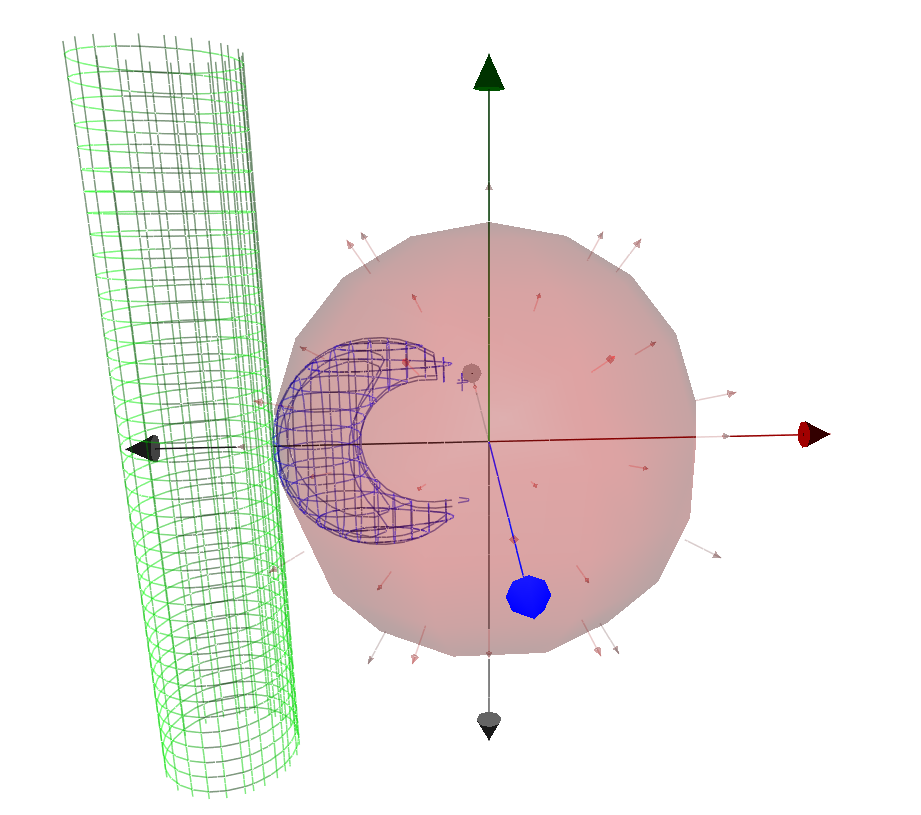
\includegraphics[scale=0.4]{ReflectCylinderInSphere}
\caption{The blue reflection of a green cylinder in a red sphere.  Traces in various planes were
used to render the cylinder and reflection surfaces.  Numerical instability in the tracing algorithm
leads to problems in drawing the part of the reflected surface near the origin.}
\label{fig_reflect_cylinder_in_sphere}
\end{figure}
The functions beginning with the word ``bind'' create and bind an entity to the given
element of the geometric algebra that is responsible for interpreting that element
as a surface under Definition~\ref{def_surface} or as a surface under the definition
given by the conformal model.  The computer program can then
use traditional methods to render the surface from the extracted polynomial equation.
For example, the polynomial equation in $x$, $y$ and $z$ for the reflected surface presented
in Figure~\ref{fig_reflect_cylinder_in_sphere} is given by
\begin{equation}
\begin{split}
0 =\;& 28.8x^{2} + 11.2x^{3} + x^{4} + 11.2xy^{2} + 2x^{2}y^{2} + \\
 & 11.2xz^{2} + 2x^{2}z^{2} + y^{4} + 2y^{2}z^{2} + 28.8z^{2} + z^{4}.
\end{split}
\end{equation}
It is interesting how a bit of reasoning in geometric algebra has given us a means
to finding this polynomial equation.
Of course, while such equations lend themselves to computer algorithms, they
are not practical on paper.  This is where the canonical forms of elements become
useful.  A parameterization of the reflected surface of Figure~\ref{fig_reflect_cylinder_in_sphere} in terms
of lengths, vectors and positions, however, does not seem obvious, but is plausible and surely exists.

\nocite{Dorst07}
\bibliographystyle{amsplain}
\bibliography{Parkin_AnExtensionOfTheQuadricModel}

\end{document}